\section{Supplementary Material}\label{sec:supp_material}

\paragraph{Simplicial distance and the localizing property of the Laplacian.}
Suppose that $\sigma$ and $\tau$ are $p$-simplices for which $(\nu_0, \nu_1, \dotsc, \nu_d)$ is the shortest sequence of $p$-simplices with the property that $\nu_0=\sigma$, $\nu_d=\tau$, and each $\nu_i$ shares a face or a coface with $\nu_{i-1}$, and a face or a coface with $\nu_{i+1}$. We say that $d$ is the \emph{simplicial distance} between $\sigma$ and $\tau$. Then for all $N<d$, the entry of $L_p^N$ corresponding to $\sigma$ and $\tau$ is $0$, and so the filter does not cause interaction between $c(\sigma)$ and $c(\tau)$. This is analogous to a size-$d$ ordinary CNN layer not distributing information between pixels that are more than $d$ pixels apart. We will refer to $N$ as the \emph{degree} of the convolutional layer, but one may well wish to keep in mind the notion of \emph{size} from traditional CNNs.

\paragraph{Co-authorship complexes.}
Given a set of papers with their respective authors, a co-authorships complex is built by adding a $(k-1)$-simplex for each paper with $k$ authors. Differently from hypergraphs, simplicial complexes are closed under subsets. This means that when one adds a $(k-1)$-simplex all its subsimplices are included. The added subsimplices represent collaborations among subgroups of the authors in writing the same paper. For this reason simplicial complexes seem the natural mathematical framework to encode $n$-fold interactions. In this article we focused on co-authorship complexes, in a more general setting a simplicial complex representing $n$-fold interactions can be constructed as the one-mode projection of a bipartite graph. Namely, given a bipartite graph $X$-$Y$, the simplicial projection on $Y$ is the simplicial complex whose $(k-1)$-simplices are sets of $k$ neighboring vertices in $Y$. For example, our co-authorships complexes are constructed as simplicial projections of the paper-author bipartite graph (see Figure~\ref{fig:bipartite}). In this setting, cochains on the simplicial projection come naturally from weights on $X$ as one can define a cochain on a $k$-simplex as a function of the weights of the vertices of $X$. Specifically, given any $(k-1)$-simplex $[y_1,\dots,y_k]$ and its neighbor vertices $\{x_1,\dots,x_j\}\subseteq X$ one can define a $k$-cochain as $\phi(\{x_1,\dots,x_j\})$, for any function $\phi: \mathcal{P(X)}\longrightarrow \RR $. In our case, the function is the sum and the wights are given by the number of citations (see Figure~\ref{fig:bipartite}).

\begin{figure}[htpb]
%\begin{table*}[!t]
\savebox{\tempbox}{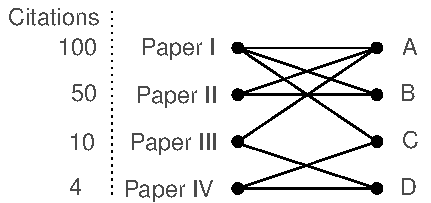
\includegraphics[height=2.3cm]{./figures/bipartite.pdf}}%
\settowidth{\tempwidth}{\usebox{\tempbox}}%
\hfil\begin{minipage}[b]{\tempwidth}%
\raisebox{-\height}{\usebox{\tempbox}}%
%\vspace{-7pt}
\scriptsize{\caption*{(a)}}%
\end{minipage}%
\savebox{\tempbox}{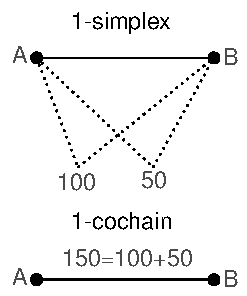
\includegraphics[height=2.5cm]{./figures/cochain.pdf}}%
\settowidth{\tempwidth}{\usebox{\tempbox}}%
\hfil\begin{minipage}[b]{\tempwidth}%
\raisebox{-\height}{\usebox{\tempbox}}%
\scriptsize{\captionof*{figure}{(b)}}%
\end{minipage}%
\vspace{5pt}
%\end{table*}
\savebox{\tempbox}{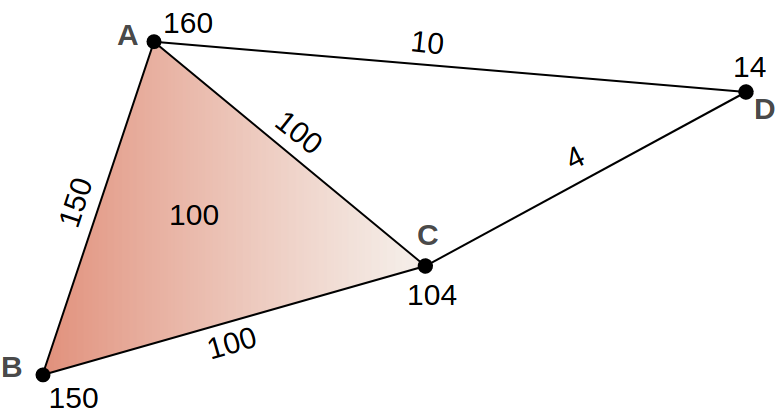
\includegraphics[height=2.5cm]{./figures/cc1.png}}%%
\settowidth{\tempwidth}{\usebox{\tempbox}}%
\hfil\begin{minipage}[b]{\tempwidth}%
\raisebox{-\height}{\usebox{\tempbox}}%
\scriptsize{\captionof*{figure}{(c)}}%
\end{minipage}%
%\end{table*}
\caption{Constructing a simplicial complex and its cochain from a bipartite graph. (a) Paper-author bipartite graph using the data of Figure~\ref{fig:data2complex}. (b)The $2$-simplex $[A,B]$ is included in the co-authorship complex sinece $A$ and $B$ are $2$ neighbor. The cochain on $[A,B]$ is given by the sum of the citations on the neighboring papers. (c) Co-authorship complex with cochains built from the citations on papers.}\label{fig:bipartite}
\end{figure}



We report in the following table the number of simplices in dimension $k=0,1,2$ of the co-authorship complexes CC1 and CC2. In Figure~\ref{fig:dist-cochains} we show the distribution of the values of the cochains in CC1 and CC2.
\begin{table}[htbp]
  \centering
  \scriptsize{
  \begin{tabular}{lrrrrrrrrrrr}
    \toprule
    Dimension   & 0     & 1  & 2     & 3 & 4     & 5 & 6    & 7 & 8   & 9 & 10\\
    \midrule
    CC1 & 352  & 1474  & 3285  & 5019  & 5559  & 4547  & 2732  & 1175  & 343 & 61 & 5\\
    CC2 & 1126 & 5059 & 11840 & 18822 & 21472 & 17896  & 10847 & 4673 & 1357 & 238 & 19\\
    \bottomrule
  \end{tabular}}
  \vspace{2pt}
  \caption{%
  Number of simplices of the two co-authorship complexes sampled from Semantic Scholar.
  } \label{table:Simplices-coauthor}
\end{table}

\begin{figure}[tb]
\centering
 \begin{subfigure}[t]{-0.8\textwidth}
 \vspace{-4cm}
    \text{(a)}
  \end{subfigure}
\begin{subfigure}[t]{0.8\textwidth}
\centering
   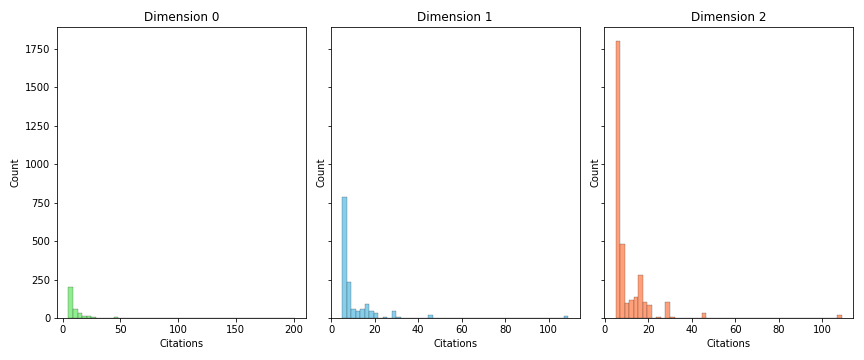
\includegraphics[scale=0.26]{./figures/distribution_cochain_150250.png}
 %\caption{Accuracy of SNN in predicting missing citations } \label{fig:accuracy}
\end{subfigure}
 \begin{subfigure}[t]{0.8\textwidth}
    \text{(b)}
  \end{subfigure}
\begin{subfigure}[t]{0.8\textwidth}
\centering
\vspace{-0.5cm}
   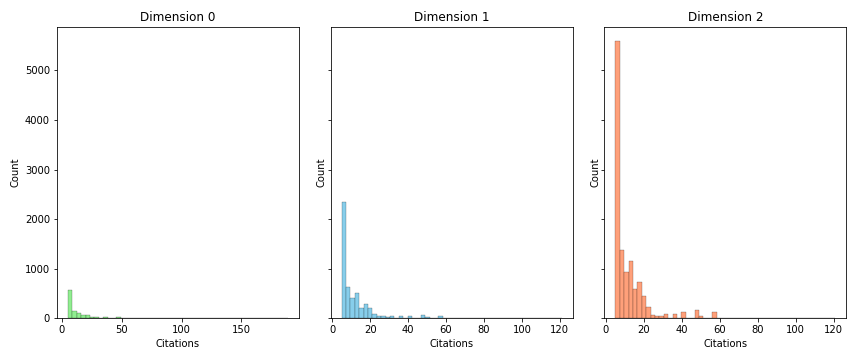
\includegraphics[scale=0.26]{./figures/distribution_cochain_11779.png}
 % \caption{Distribution of the prediction's error} \label{fig:error}
\end{subfigure}
\caption{(a) Distribution of the $k$-cochain values on CC1 ($k=1,2,3$). (b) Distribution of the $k$-cochain values on CC2 ($k=1,2,3$).}
\label{fig:dist-cochains}
\end{figure}

\paragraph{Glossary Missing Data Imputation.}
We state here some definitions and criteria that are used in the results section.
A missing value is predicted correctly if the imputed value differs of at most $1$ from the actual values. \mdeff{Shouldn't that be relative? Being off by 1 citation is different for 5 and 1000 citations.}\stefania{I agree. What would you take as a relative threshold to be considered correct?$10\%$?I recompute the accuracy with the decided value.}
The \emph{accuracy} is defined as the percentage of missing values that has been correctly imputed and the \emph{absolute error} (AE) as the magnitude of the difference between the predicted and actual citation.
For the same percentage of missing values we consider different random samples of the damaged portions. Then a statistical evaluation of the performance of the network is given by the \emph{mean accuracy} (MA), the mean of the accuracy over different samples.

\stefania{Write acknowledgments: add Kathryn @Micheal do you wanna add someone? }
